\documentclass[12pt,landscape]{article}

%Incantation for swapping landscape/seascape
\special{! TeXDict begin /landplus90{true}store end }

\usepackage[utf8]{inputenc}
\usepackage{amssymb}
\usepackage{stmaryrd}
\usepackage{textcomp}
\usepackage[cm]{fullpage}
\usepackage{color}
\usepackage{t1enc}
\usepackage{amsmath}
\usepackage{url}
\usepackage{graphics}
\usepackage[all]{xy}
\usepackage{tikz, tikz-cd}
% Use the patterns library to draw the cubes figure
\usetikzlibrary{patterns}
\xyoption{2cell}
\UseAllTwocells

\newcommand\whitecol[1]{\textcolor{white}{#1}}


% Color palette
\RequirePackage{xcolor}

\definecolor{white}{HTML}{FFFFFF}
\definecolor{gray80}{rgb}{0.2, 0.2, 0.2}
\definecolor{gray65}{rgb}{0.35, 0.35, 0.35}
\definecolor{gray30}{rgb}{0.70, 0.70, 0.70}
\definecolor{raspeberry}{HTML}{BF3343}
\definecolor{strawberry}{HTML}{D86E7A}
\definecolor{hlcolor}{HTML}{FBEFF1}
\definecolor{yaleblue}{HTML}{054A91}

% Color palette 2
\definecolor{russian-green}{HTML}{69995D}
\definecolor{chestnut}{HTML}{98473E}
\definecolor{indian-yellow}{HTML}{DB9D47}
\definecolor{carolina}{HTML}{009FFD}
\definecolor{spanish-blue}{HTML}{296EB4}

\makeatletter
\newcommand{\Overrightarrow}[2]{\raisebox{#1}{$\ext@arrow 0359\Rightarrowfill@{\mbox{${#2}$}}{}$}}
\newcommand{\Overleftarrow}[2]{\raisebox{#1}{$\ext@arrow 0359\Leftarrowfill@{\mbox{${#2}$}}{}$}}
%\newcommand{\Overrightarrow}[1]{\raisebox{1.4ex}{$\ext@arrow 0359\Rightarrowfill@{\mbox{${#1}$}}{}$}}
\makeatother

\newenvironment{myitemize}
{\begin{list}{}{
  % Horizontal spaces
%  \setlength{\rightmargin}{0pt} % ?
%  \setlength{\listparindent}{0pt} % ?
  \setlength{\labelwidth}{5pt} % Global indentation reserved for label
  \setlength{\labelsep}{5pt} % How far is the label on the left of paragraph
  \setlength{\leftmargin}{10pt} % should be labelwidth + labelsep
  \setlength{\parindent}{0pt} % Indentation of next paragraphs of the item
  \setlength{\itemindent}{0pt} % Indentation of the first line of item
  % Vertical spaces
  \setlength{\parskip}{8pt} % Distance between two paragraphs or item
  \setlength{\itemsep}{2pt} % Extra distance between two items
  \setlength{\parsep}{10pt}}}
{\end{list}}

\newcommand{\highlight}[1]{{\em #1}}

\newcommand{\Type}{\mathsf{Type}}
\newcommand{\Set}{\mathsf{Set}}
\newcommand{\Prop}{\mathsf{Prop}}
\newcommand{\refl}[1]{\mathsf{refl}\,{#1}}
\newcommand{\mkmlidtype}[3]{{#1} =^{\mathrm{id}}_{#2} {#3}}
\newcommand{\mkmleqdep}[3]{{#1} =^{\mathrm{dep}}_{#2} {#3}}
\newcommand{\hrefl}[1]{\mathsf{refl^{\mathrm{dep}}}\,{#1}}
\newcommand{\mluniv}{\mathsf{U}}
\newcommand{\Jdep}[2]{\mathsf{J}\;{#1}\;{#2}}

\newcommand{\nth}[1]{{#1}^{\mbox{\scriptsize th}}}
\newcommand{\binomial}[2]{\left(\begin{array}{c}#1\\#2\end{array}\right)}

\newcommand{\wfctx}[1]{{#1}~\mathsf{ok}}

\newcommand{\mkover}[1]{\widetilde{#1}}
\newcommand{\mkoverdim}[2]{\widetilde{#2}^{#1}}
%\newcommand{\mkover}[1]{\dot{#1}}
\newcommand{\mkprod}[3]{\Pi {#1}\!:\!{#2}.\,{#3}}
\newcommand{\mkprodovereq}[3]{\mkover{\Pi} {#1}\!:\!{#2}.\,{#3}}
\newcommand{\mkprodovereqopp}[3]{\opp{\mkover{\Pi}} {#1}\!:\!{#2}.\,{#3}}
\newcommand{\mkboundedprod}[4]{\Pi {#3}\!:\!{#1}\leq{#2}.\,{#4}}
\newcommand{\mklam}[3]{\lambda {#1}\!:\!{#2}.\,{#3}}
\newcommand{\mkboundedlam}[4]{\lambda {#3}\!:\!{#1}\leq{#2}.\,{#4}}
\newcommand{\mkapp}[2]{{#1}\,{#2}}
\newcommand{\prodsort}[2]{\Pi ({#1},{#2})}

% selecting kind of treatment of sorts
\newcommand{\typeorsort}[2]{{#2}}

\newcommand{\mksigma}[3]{\Sigma {#1}\!:\!{#2}.\,{#3}}
\newcommand{\mksigmaovereq}[3]{\mkover{\Sigma} {#1}\!:\!{#2}.\,{#3}}
\newcommand{\mksigmaovereqopp}[3]{\opp{\mkover{\Sigma}} {#1}\!:\!{#2}.\,{#3}}
\newcommand{\mkpair}[2]{\langle{#1},{#2}\rangle}
\newcommand{\mkfst}[1]{{#1}.1}
\newcommand{\mksnd}[1]{{#1}.2}
\newcommand{\sigsort}[2]{\Sigma ({#1},{#2})}

\newcommand{\sortsort}[1]{{\mathcal S}_{#1}}

\newcommand{\Sone}{\mathbb{S}^1}
\newcommand{\casesone}[5]
  {\mathsf{case}\;{#1}\;\mathsf{of}\;{#2}\;\Rightarrow\;{#3}\;|\;{#4}\;\Rightarrow\;{#5}\;\mathsf{end}}
\newcommand{\base}{\mathsf{base}}
\newcommand{\loopsone}{\mathsf{loop}}
\newcommand{\Sonesort}{l_{\mathbb{S}^1}}

\newcommand{\emptyctx}{\emptyset}

\newcommand{\sort}[1]{\mathsf{Type}_{#1}}
\newcommand{\istype}{~:~\mluniv}

\newcommand{\mkeq}[3]{{#1} =_{#2} {#3}}
\newcommand{\mkhomeq}[3]{{#1} =_{#2} {#3}}
\newcommand{\mkeqovereq}[3]{{#1} \,\mkover{=}_{#2}\, {#3}}
\newcommand{\mkeqovereqdim}[4]{{#2} \,\mkoverdim{#1}{=}_{#3}\, {#4}}
\newcommand{\mkeqtype}[3]{{#1} =_{#2} {#3}} % case where we can write either s or refl{s}
\newcommand{\mkeqtypeovereq}[3]{{#1} \,\mkover{=}_{#2}\, {#3}} % case where we can write either s or refl{s}
\newcommand{\mkeqarray}[3]{\begin{array}{c}{#1}\\ =_{#2}\\ {#3}\end{array}}
\newcommand{\mkfaces}[3]{\mkeq{#1}{#2}{#3}}
\newcommand{\mkfacesarray}[3]{\mkeqarray{#1}{#2}{#3}}
\newcommand{\mkfacesover}[3]{\mkeqovereq{#1}{#2}{#3}}
\newcommand{\lameq}[2]{\lambda {#1}.{#2}}
%\newcommand{\reflterm}[1]{\textsf{refl}{#1}}
\newcommand{\reflterm}[1]{\widehat{#1}}
\newcommand{\overreflterm}[1]{{\mkover{\reflterm{#1}}}}
\newcommand{\minirefltermdim}[2]{{{\widehat{#2}}^{\raisebox{1mm}{\normalsize #1}}}}
\newcommand{\refltermdim}[2]{\widehat{#2}^{#1}}
%\newcommand{\reflterm}[1]{\lambda{#1}}
%\newcommand{\refltype}[1]{\lambda{#1}}
\newcommand{\refltype}[1]{\reflterm{#1}}
\newcommand{\purerewlr}[1]{\overrightarrow{#1}}
\newcommand{\purerewrl}[1]{\overleftarrow{#1}}
%\newcommand{\rewlr}[2]{\mathsf{rew}^\rightarrow\;{#1}\;\mathsf{in}\;{#2}}
%\newcommand{\rewrl}[2]{\mathsf{rew}^\leftarrow\;{#1}\;\mathsf{in}\;{#2}}
\newcommand{\rewlrmap}[1]{\overrightarrow{#1}}
\newcommand{\rewrlmap}[1]{\overleftarrow{#1}}
\newcommand{\rewlr}[2]{\overrightarrow{#1}(#2)}
\newcommand{\rewrl}[2]{\overleftarrow{#1}(#2)}
\newcommand{\deprewlr}[1]{\raisebox{0em}{$\ulcorner$}\!#1}
\newcommand{\minideprewlr}[1]{\raisebox{0em}{$\ulcorner$}\!\!\!#1}
\newcommand{\deprewrl}[1]{{#1}\raisebox{-0.2em}{$\!\lrcorner$}}
\newcommand{\rewlrspec}[2]{{#1}^{\rightarrow}(#2)}
\newcommand{\rewrlspec}[2]{{#1}^{\leftarrow}(#2)}
\newcommand{\rewlrrevspec}[2]{{#1}_-^{\rightarrow}(#2)}
\newcommand{\rewrlrevspec}[2]{{#1}_-^{\leftarrow}(#2)}
\newcommand{\rewlrrevspecin}[2]{{#1}_+^{\rightarrow}(#2)}
\newcommand{\rewrlrevspecin}[2]{{#1}_+^{\leftarrow}(#2)}
\newcommand{\doublerewlr}[2]{\Overrightarrow{1.4ex}{#1}({#2})}
\newcommand{\doublerewrl}[2]{\Overleftarrow{1.4ex}{#1}({#2})}
\newcommand{\doublerewlrmap}[1]{\Overrightarrow{1.4ex}{#1}}
\newcommand{\doublerewrlmap}[1]{\Overleftarrow{1.4ex}{#1}}
\newcommand{\cohrewlr}[2]{\mathsf{coh}{#1}({#2})}
%\newcommand{\mktuple}[6]{\{#1\mapsto #3(#1); #2\mapsto #4(#2); #1\mapsto #5(#1); #2\mapsto #6(#2)\}}
\newcommand{\mktuple}[6]{\{#3; #4; #5; #6\}_{#1,#2}}
\newcommand{\mkcohtuple}[7]{\{#3; #4; #5; #6; #7\}_{#1,#2}}
\newcommand{\mktupleshort}[6]{\{#3; #4; #5; #6\}}
\newcommand{\mktupleshortnamed}[6]{\{#3; #4; #5; #6\}_{#1,#2}}
\newcommand{\opp}[1]{{#1}^{-1}}
\newcommand{\oppi}[2]{\appi{#1}{(\opp{#2}/{#2})}}

\newcommand{\weakensquarelr}[1]{{#1}_L}
\newcommand{\weakensquarerl}[1]{{#1}_R}
\newcommand{\weakensquarelrmap}[1]{{#1}_L}
\newcommand{\weakensquarerlmap}[1]{{#1}_R}

\newcommand{\rewlrmkeq}[4]{\mkeq{\rewlr{#1}{#2}}{#3}{#4}}

% Version basse
%% \newcommand{\appi}[2]{{#1}_{#2}}
%% \newcommand{\appidep}[2]{{#1}_{({#2})}}
%% \newcommand{\bp}[1]{{#1}_0}
%% \newcommand{\ep}[1]{{#1}_1}
%% \newcommand{\bpdep}[1]{{#1}_{(0)}}
%% \newcommand{\epdep}[1]{{#1}_{(1}}}
% Version haute
% \newcommand{\metaappi}[2]{{#1}_{[{#2}]}}
\newcommand{\appi}[2]{{#1}\;\!{#2}}
\newcommand{\appidep}[2]{{#1}_{#2}}
\newcommand{\bp}[1]{{#1}{\scriptstyle 0}}
\newcommand{\ep}[1]{{#1}{\scriptstyle 1}}
\newcommand{\bpoverdim}[2]{{#2}{\scriptstyle \mkoverdim{#1}{0}}}
\newcommand{\epoverdim}[2]{{#2}{\scriptstyle \mkoverdim{#1}{1}}}
\newcommand{\bpdep}[1]{{#1}_0}
\newcommand{\epdep}[1]{{#1}_1}

\newcommand{\bpsubstexpl}[2]{{#2}_{\{0/{#1}\}}}
\newcommand{\epsubstexpl}[2]{{#2}_{\{1/{#1}\}}}
\newcommand{\eqsubstexpl}[2]{{#2}_{\{\star/{#1}\}}}
\newcommand{\bpsubstexplcons}[2]{{#2}\}\{0/{#1}}
\newcommand{\epsubstexplcons}[2]{{#2}\}\{1/{#1}}
\newcommand{\eqsubstexplcons}[2]{{#2}\}\{\star/{#1}}
\newcommand{\bpsubst}[2]{{#2}{[0/{#1}]}}
\newcommand{\epsubst}[2]{{#2}{[1/{#1}]}}
\newcommand{\bpsubstctx}[3]{{#3}{[0/{#2}]}^{#1}}
\newcommand{\epsubstctx}[3]{{#3}{[1/{#2}]}^{#1}}
\newcommand{\takebpface}[2]{\partial^{#1}_0{#2}}
\newcommand{\takeepface}[2]{\partial^{#1}_1{#2}}

\newcommand{\dimvalid}[2]{{#1} \in {#2}}
\newcommand{\dimdeclare}[1]{{#1}}
\newcommand{\dimlength}[1]{|#1|_{\mathit{dim}}}
\newcommand{\dimindex}[2]{\#_{#1}{#2}}

\newcommand{\substminus}[2]{{#1}-{#2}}
\newcommand{\substminusbernardymoulin}[2]{{#1}/{#2}}

\newcommand{\N}{\mathbb{N}}
\newcommand{\expand}[2]{\mathsf{expand}(#1,#2)}

\newcommand{\defeq}{\triangleq}
%\newcommand{\metaequiv}{=\!\!\!=}
\newcommand{\metaequiv}{\cong}
\newcommand{\metaletin}[3]{\mathit{let}\;{#1}\;\defeq\;{#2}\;\mathit{in}\;{#3}}
\newcommand{\map}[2]{\mathsf{ap}\,{#1}\,{#2}}
\newcommand{\depmap}[2]{\mathsf{apd}\,{#1}\,{#2}}
\newcommand{\transport}[3]{\mathsf{transport}\,{#1}\,{#2}\,{#3}}
\newcommand{\deptransport}[3]{\mathsf{transportd}\,{#1}\,{#2}\,{#3}}
%\newcommand{\swap}[1]{\mathsf{swap}(#1)}
%\newcommand{\swapbracket}[1]{\mathsf{swap}(#1)}
%\newcommand{\swaptype}[1]{\mathsf{swap}(#1)}
\newcommand{\swap}[1]{{#1}^{\circ}}
\newcommand{\swapbracket}[1]{({#1})^{\circ}}
\newcommand{\swaptype}[1]{{#1}^{\circ}}
\newcommand{\swapoverdim}[2]{{#2}^{\mkoverdim{#1}{\circ}}}
\newcommand{\homsquare}[1]{\mathsf{homsquare}(#1)}
\newcommand{\permute}[2]{\mathsf{permute}_{#1}(#2)}
\newcommand{\adjacenttranspose}[2]{\sigma_{#1}({#2})}
\newcommand{\swapprodeq}[2]{\mathsf{swap}_{\Pi=}^{#1}(#2)}
\newcommand{\swapeqprod}[2]{\mathsf{swap}_{=\Pi}^{#1}(#2)}
\newcommand{\swapeqprodlr}[2]{\mathsf{swap}_{=\Pi}^{\rightarrow}({#1})(#2)}
\newcommand{\swapeqprodrl}[2]{\mathsf{swap}_{=\Pi}^{\leftarrow}({#1})(#2)}
\newcommand{\swapsigmaeq}[1]{\mathsf{swap}_{\Sigma=}(#1)}
\newcommand{\swapeqsigma}[1]{\mathsf{swap}_{=\Sigma}(#1)}

\newcommand{\bool}{\mathsf{bool}}
\newcommand{\booldeux}{\bool^2}
\newcommand{\boolexp}{\bool^{\bool}}

\newcommand{\reduce}{\;\triangleright\;}

\newcommand{\emptysubst}{\emptyctx}

\newcommand{\sortrule}{\sort{}}
\newcommand{\axrule}{\mathsf{Ax}}
\newcommand{\ctxemptyrule}{\mathsf{Ctx}_{\emptyctx}}
\newcommand{\ctxconsrule}{\mathsf{Ctx}_{\mathsf{cons}}}
\newcommand{\convrule}{\mathsf{Conv}}
\newcommand{\convruleredright}{\reduce_R}
\newcommand{\convruleredleft}{\reduce_L}
\newcommand{\convrulerefl}{\equiv_{\mathsf{refl}}}
\newcommand{\convruletrans}{\equiv_{\mathsf{trans}}}

\newcommand{\circovereq}{\;\mkover{\circ}\;}
\newcommand{\circsigma}{\circ_{\Sigma}}

\newcommand{\comprule}{R_{\mathsf{\circ}}}
\newcommand{\opprule}{R_{\mathsf{\opp}}}

\newcommand{\idleftredrule}{\mathsf{Id_L}}
\newcommand{\idrightredrule}{\mathsf{Id_R}}
\newcommand{\idoppredrule}{\mathsf{\opp{Id}}}
\newcommand{\oppoppredrule}{\mathsf{\opp{(\opp{\_})}}}
\newcommand{\assoccompredrule}{\mathsf{Assoc}}
\newcommand{\distriboppcompredrule}{\mathsf{\opp{\circ}}}
\newcommand{\squaredownredrule}{\circ_{=_{\mkover{=}}}}
\newcommand{\exchangerule}{\mathsf{Exch}}
\newcommand{\compeqovereqredrule}{\circ_{\mkover{=}}}
\newcommand{\squareprodredrule}{\circ_{=_{\mkover{\Pi}}}}

\newcommand{\depmapdef}{\mathsf{ApD}}
\newcommand{\funextpuredef}{\mathsf{LiftDim}}
\newcommand{\funextdeppuredef}{\mathsf{LiftDepDim}}
\newcommand{\funextdepdeppuredef}{\mathsf{LiftDepDim}}
\newcommand{\funextdef}{\mathsf{FunExt}}
\newcommand{\funextdepdef}{\mathsf{FunDepExt}}
\newcommand{\funext}[1]{\mathsf{funext}(#1)}
\newcommand{\funextdep}[1]{\mathsf{fundepext}(#1)}
\newcommand{\funextpure}[1]{\mathsf{liftdim}(#1)}
\newcommand{\funextdeppure}[1]{\mathsf{liftdepdim}(#1)}

\newcommand{\partialcubset}[2]{\mathsf{\nu set}_{#1}^{<#2}}
\newcommand{\mycubset}[1]{\mathsf{\nu set}_{#1}}
\newcommand{\mycubsetfrom}[2]{\mathsf{\nu set}_{#1}^{\geq#2}}
\newcommand{\mycubsetcomp}[2]{\mathsf{\nu set}_{#1}^{=#2}}
\newcommand{\mybox}[1]{\mathsf{frame}_{#1}}
\newcommand{\mylayer}[1]{\mathsf{layer}_{#1}}
\newcommand{\mycube}[1]{\mathsf{painting}_{#1}}
\newcommand{\myfullbox}[1]{\mathsf{fullframe}_{#1}}
\newcommand{\unitpoint}{\star}
\newcommand{\unittype}{\mathsf{unit}}
\newcommand{\hd}{\mathsf{hd}}
\newcommand{\tl}{\mathsf{tl}}
\newcommand{\downbox}[2]{\mathsf{restrframe}_{#1,#2}}
\newcommand{\downlayer}[2]{\mathsf{restrlayer}_{#1,#2}}
\newcommand{\downcube}[2]{\mathsf{restrpainting}_{#1,#2}}
\newcommand{\cohbox}[2]{\mathsf{cohframe}_{#1,#2}}
\newcommand{\cohlayer}[2]{\mathsf{cohlayer}_{#1,#2}}
\newcommand{\cohcube}[2]{\mathsf{cohpainting}_{#1,#2}}


\newcommand{\mkeqsquare}[5]{\begin{array}{c}{#1} ~~=~~ {#5}\\[-0.2cm] ~~\mbox{}_{\mkeqovereq{#2}{#3}{#4}}\\\end{array}}
\newcommand{\mkeqcube}[7]{\begin{array}{c}{#1} ~~=~~ {#7}\\[-0.2cm] ~~\mbox{}_{#2~\mkover{=}~#6}\\[-0.2cm] ~~~~~\;\mbox{}_{\mbox{}_{\mkeqovereqdim{2}{#3}{#4}{#5}}}\\\end{array}}
\newcommand{\xysquare}[9]{
  \xymatrix{
  {#1} \ar_{#5}[dd] \ar^{#7}[rrr] & & & \ar^{#6}[dd] {#3}\\
  *\txt<4pc>{} \ar^{#9}@{=>}[rrr] & & & *\txt<4pc>{}\\
  {#2} \ar^{#8}[rrr] & & & {#4}}
}

\begin{document}
\begin{Large}
\begin{sf}

\mbox{}
\vspace{3cm}

\begin{center}

\textcolor{red}{\Huge About the construction of simplicial and cubical
  sets in indexed form: the case of degeneracies}

\medskip
\bigskip
\bigskip
{\Large Hugo Herbelin} \\
\bigskip
{\Large Ramkumar Ramachandra}

\bigskip
\bigskip
\bigskip
\bigskip
\bigskip
\bigskip
\bigskip
TYPES 2025

\bigskip
\bigskip
Glasgow
\bigskip

10 June 2025

\bigskip
\bigskip

\end{center}


%%%%%%%%%%%%%%%%%%%%%%%%%%%%%%%%%%%%%%%%%%%%%%%%%%%%%%%%%%%%%%%%%%%%%%
\newpage

\begin{center}
\textcolor{red}{\huge Outline}
\end{center}

\bigskip
\noindent - Reedy presheaves in (usual) fibered form vs indexed form, why?
\bigskip

\noindent - unary and binary parametricity as a language to uniformly talk about respectively augmented simplicial and cubical sets
\bigskip

\noindent - simplicial degeneracies are actually not a unary form of cubical
degeneracies but of connections
\bigskip

\noindent - an effective uniform indexed construction of augmented simplicial and cubical sets with one degeneracy (machine-checked in Rocq)

%% \mbox{}

%% \vspace{5cm}

%% \begin{center}
%% \textcolor{red}{\huge Investigations into syntactic iterated parametricity and cubical type theory
%% Towards syntactic ``indexed'' models of various cubical/parametric type theories}
%% \end{center}

\newcommand{\mysem}[1]{\llbracket #1 \rrbracket}
\newcommand{\deppsh}[2]{\mathsf{DepPresheaf}(#1,#2)}
\newcommand{\HSet}{\mathsf{HSet}}

\iffalse
%%%%%%%%%%%%%%%%%%%%%%%%%%%%%%%%%%%%%%%%%%%%%%%%%%%%%%%%%%%%%%%%%%%%%%
\newpage

\begin{center}
\textcolor{red}{\huge Presheaf models of homotopy type theory in indexed form: motivation}
\end{center}

\bigskip

Different approaches, different traditions:
\bigskip

\begin{tabular}{ccc}
``Semantic'' (presheaf) models & vs & ``Syntactic'' models\\
\\
$
\begin{array}{l}
\vdash_{ZF} ((\Gamma \vdash_{TT} A) \rightarrow \deppsh{\Gamma}{A})\\
\vdash_{TT} ((\Gamma \vdash_{TT} A) \rightarrow \deppsh{\Gamma}{A})\\
\end{array}
$ & &
$\vdash_{PRA} ((\Gamma \vdash_{TT} A) \rightarrow (\vdash_{ETT} \deppsh{\Gamma}{A})$\\
\\
& & separation of concerns \\
close to the ``mental'' intuitions & &
protects from a ``set-theoretic'' bias\\
& & metalanguage does not leak\\
\end{tabular}

\bigskip
Reedy presheaves in (usual) ``fibred'' form vs Reedy presheaves in ``indexed'' form

Advantages:
Relatively simple definition
Well-studied

Advantages:
Closer to the syntax, liable to better preserve definitional equalities
Interesting in itself
\fi

%%%%%%%%%%%%%%%%%%%%%%%%%%%%%%%%%%%%%%%%%%%%%%%%%%%%%%%%%%%%%%%%%%%%%%
\newpage

\begin{center}
\textcolor{red}{\huge The fibred/indexed correspondence for h-sets}
\end{center}

\bigskip
For $B:\HSet_l$

$$\Sigma E:\HSet_l.\, (E \rightarrow B) ~\simeq~ B \rightarrow \HSet_l$$

\bigskip

Application to the definition of Reedy presheaves in \emph{indexed form}, here for cubical sets:

$$
\begin{array}{cllccllll}
\multicolumn{3}{c}{\mbox{\emph{fibred form}}} & \qquad\mathit{vs}\qquad & \multicolumn{3}{l}{\mbox{\emph{indexed form}}} \\
\\
Y_0 &:& \HSet_l & & X_0 & : & \HSet_l & \mbox{(points)}\\
\uparrow\uparrow \\
Y_1 &:& \HSet_l & & X_1 & : & X_0 \times X_0 \rightarrow \HSet_l & \mbox{(segments)}\\
\uparrow\uparrow\uparrow\uparrow \\
Y_2 &:& \HSet_l & & X_2 & : & \Pi (x_{LL},x_{LR}):(X_0 \times X_0).\, \Pi x_{L*}:X_1 (x_{LL},x_{LR}).\\
& & & & & & \Pi (x_{RL},x_{RR}):(X_0 \times X_0).\, \Pi x_{R*}:X_1 (x_{RL},x_{RR}).\, \\
\multicolumn{3}{c}{\mbox{~+ coherences}} & & & & X_1 (x_{LL},x_{RL}) \times X_1 (x_{LR},x_{RR}) \rightarrow \HSet_l \qquad & \mbox{(squares)}\\
\\
\vdots & & & & \vdots\\
\end{array}
$$

%%%%%%%%%%%%%%%%%%%%%%%%%%%%%%%%%%%%%%%%%%%%%%%%%%%%%%%%%%%%%%%%%%%%%%
\newpage

\begin{center}
\textcolor{red}{\huge Building presheaves in indexed form directly}
\end{center}

\bigskip

Alternatively, we can define ``matching objects''
$M_n(X_0,...,X_{n-1})$ directly on the indexed side without referring
first to the fibred side. This was done, e.g., for semi-simplicial sets:

\begin{itemize}
\item By defining matching object as the collection of
  all faces, quotiented with $M_{f \circ g} = M_f \circ M_g$, as
  in Voevodsky 2012, Part and Luo 2015, Altenkirch, Capriotti and Kraus 2016, ...
\item By relying on specific presentations of a category:
\begin{itemize}
\item The $d^n_i$ generators and $d_id_j = d_{j-1}d_i$ coherences in H. 2013
\item By following parametricity rules in H. and Ramachandra 2025
\end{itemize}
\end{itemize}

\vspace{5cm}

Eventually expecting interpretations, e.g. of the universe, that more closely follow the syntax...

\iffalse
%%%%%%%%%%%%%%%%%%%%%%%%%%%%%%%%%%%%%%%%%%%%%%%%%%%%%%%%%%%%%%%%%%%%%%
\newpage

\begin{center}
\textcolor{red}{\huge Building presheaves in indexed form directly}
\end{center}

The indexed definitions may look more complicated (the indexed
definition is in charge of ensuring the coherence laws while in the
fibred case, only concrete instances of presheaf are in charge to do so)

The indexed definition is expected to have specific definitional
property. For instance, a (cubical) line between presheaves $A$ and
$B$ in the universe presheaf is not any more a presheaf over $A$ and
$B$ but a presheaf dependent over $A$ and $B$, the same way as $A
\times B \rightarrow \sort{}$ would be (intuitively) interpreted.
\fi

%%%%%%%%%%%%%%%%%%%%%%%%%%%%%%%%%%%%%%%%%%%%%%%%%%%%%%%%%%%%%%%%%%%%%%
\newpage

\begin{center}
\textcolor{red}{\huge Iterated parametricity as a uniform approach to both augmented simplicial sets and cubical sets}
\end{center}

It seems now established that the augmented simplicial and cubical
categories only differ in the ``arity'' of a finite set $\nu$:

\newcommand{\Obj}{\ensuremath{\mathsf{Obj}}}
\newcommand{\Hom}{\ensuremath{\mathsf{Hom}}}
\newcommand{\id}{\ensuremath{\mathsf{id}}}
$$
  \begin{array}{ll}
    \Obj       & := \mathbb{N}\\
    \Hom(p, n) & := \{l \in (\nu \sqcup \{\star\})^n \mid \text{number of $\star$ in $l = p$}\} \\
    g \circ f             & :=
    \begin{cases}
      f                & \text{if $g = \epsilon$}                                                   \\
      a\,(g' \circ f)  & \text{if $g = a\,g'$}, \text{where $a \in \nu$}                            \\
      a\,(g' \circ f') & \text{if $g = \star\,g'$, $f = a\,f'$, where $a \in \nu$ or $a = \star$} \\
    \end{cases}            \\
    \id                   & := \star \ldots \star \text{ $n$ times for $\id \in \Hom(n, n)$}
  \end{array}
$$

That is, we obtain:
\begin{center}
\begin{tabular}{ccc}
augmented semi-simplicial sets with $\nu = \{0\}$ & &
semi-cubical sets with $\nu = \{L,R\}$\\
\\
    e.g.: \begin{tikzcd}
      & |[alias=F]|00\star \arrow[ddr, dash, "0\star\star"] & \\\\
      \star00 \arrow[rr, dash, "\star\star0"{name=T, below}]\arrow[uur, dash, "\star0\star"] && 0\star0 \\
      \arrow[rightarrow, from=F, to=T, phantom, "\star\star\star" description]
    \end{tikzcd}
&\qquad\qquad&
    e.g.:~~~\begin{tikzcd}
      LR \arrow[r, dash, "\star R"{name=F}] \arrow[d, dash, "L\star" left] & RR \arrow[d, dash, "R\star"] \\
      LL \arrow[r, dash, "\star L"{name=T, below}] & RL \\
      \arrow[rightarrow, from=F, to=T, phantom, "\star\star" description]
    \end{tikzcd}
\end{tabular}
\end{center}

%%%%%%%%%%%%%%%%%%%%%%%%%%%%%%%%%%%%%%%%%%%%%%%%%%%%%%%%%%%%%%%%%%%%%%
\newpage

\begin{center}
\textcolor{red}{\huge Adding (one) reflexivity (in the last direction)}
\end{center}

\newcommand{\rouge}[1]{\textcolor{red}{#1}}
\newcommand{\bleu}[1]{\textcolor{blue}{#1}}

$$
\begin{array}{cllccllll}
\multicolumn{3}{c}{\mbox{\emph{fibred form}}} & \qquad\mathit{vs}\qquad & \multicolumn{3}{l}{\mbox{\emph{indexed form}}} \\
\\
Y_0 &:& \HSet_l & & X_0 & : & \HSet_l & \mbox{(points)}\\
\uparrow\uparrow\!\rouge{\downarrow} \\
Y_1 &:& \HSet_l & & X_1 & : & X_0 \times X_0 \rightarrow \HSet_l & \mbox{(segments)}\\
\uparrow\uparrow\uparrow\uparrow\!\rouge{\downarrow} &&&& \rouge{r_1} & : & \rouge{\Pi x_0:X_0.\,X_1(x_0,x_0)}\\
Y_2 &:& \HSet_l & & X_2 & : & \Pi (x^0_{LL},x^0_{LR}):(X_0 \times X_0).\, \Pi x^1_{L*}:X_1 (x^0_{LL},x^0_{LR}).\\
& & & & & & \Pi (x^0_{RL},x^0_{RR}):(X_0 \times X_0).\, \Pi x^1_{R*}:X_1 (x^0_{RL},x^0_{RR}).\, \\
\multicolumn{3}{c}{\mbox{~+ coherences}} & & & & X_1 (x^0_{LL},x^0_{RL}) \times X_1 (x^0_{LR},x^0_{RR}) \rightarrow \HSet_l \qquad & \mbox{(squares)}\\
&&&& \rouge{r_2} & : & \rouge{\Pi (x^0_{L},x^0_{R}):(X_0 \times X_0).\,\Pi x^1:X_1(x^0_L,x^0_R).}\,\\
& & & & & & \rouge{X_2((x^0_{L},x^0_{L}),r_1(x^0_{L}),(x^0_{R},x^0_{R}),r_1(x^0_{R}),(x^1,x^1))}\\
\vdots & & & & \vdots\\
\end{array}
$$

(other reflexivities can be obtained if we add also, e.g., permutations)

\bigskip

In terms of matching objects, reflexivities have the form:
$$r_n: \Pi d:M_n.\,\Pi x:X_n(d).\, X_{n+1}(M_r(d,x))$$

for some $M_r : (\Sigma d:M_n.\,X_n(d)) \rightarrow M_{n+1}$ to be defined

%%%%%%%%%%%%%%%%%%%%%%%%%%%%%%%%%%%%%%%%%%%%%%%%%%%%%%%%%%%%%%%%%%%%%%
\newpage

\begin{center}
\textcolor{red}{\huge In passing: simplicial degeneracies are
  \emph{not} the unary case of cubical degeneracies but the unary case
  of cubical \emph{connections}}
\end{center}

$\!\!\!\!\!\!\!\!\!\!\!\!\!\!\!\!\!\!$
\begin{tabular}{clll}
& \qquad \emph{set} & \qquad \emph{reflexivities} & \qquad\emph{connections} \\
& & \emph{(involve one direction)} & \emph{(involve \bleu{t}w\rouge{o} directions)} \\
\\
unary &
$\begin{array}{l}
X_{-1}:\HSet\\
X_0:X_{-1} \rightarrow \HSet\\
X_1:\Pi x^{-1}.\,\bleu{X_0(x^{-1})} \\
\quad\rightarrow \rouge{X_0(x^{-1})} \rightarrow \HSet\\
\end{array}$
 & $\begin{array}{l}
   r_{-1}:\Pi x^{-1}.X_0(x^{-1})\\
   r_0:\Pi x^{-1}.\,\Pi x^0.\, X_1(\bleu{r_{-1}(x^{-1})},\rouge{x^0})\\
   \mbox{(as in Parametric Type Theory)}\\
   \\
   \end{array}$
 & $\begin{array}{l}
  \\
   c_0:\Pi x^{-1}.\,\Pi x^0.\, X_1(\bleu{x^0},\rouge{x^0})\\
   \\
   \\
   \end{array}$\\
\\
binary &
$\begin{array}{l}
X_0 : \HSet_l\\
X_1 : X_0 \times X_0 \rightarrow \HSet_l\\
X_2 : \Pi (x^0_{LL},x^0_{LR})\bleu{x^1_{L\star}}(x^0_{RL},x^0_{RR})\bleu{x^1_{R\star }}.\\
\quad \rouge{X_1 (x^0_{LL},x^0_{RL})} \times \rouge{X_1 (x^0_{LR},x^0_{RR})}\\
\quad \rightarrow \HSet_l\\
\end{array}$
 & $\begin{array}{l}
   r_0:\Pi x^0.X_1(x^0,x^0)\\
   r_1:\Pi (x^0_L,x^0_R).\,\Pi x^1.\,\\
   \quad X_2((x^0_L,x^0_L),\bleu{r_0(x^0_L)},\\
   \quad (x^0_R,x^0_R),\bleu{r_0(x^0_{R})},\\
   \quad (\rouge{x^1},\rouge{x^1}))\\
   \end{array}$
 & $\begin{array}{l}
  \\
   c_{1L}:\Pi (x^0_L,x^0_R).\,\Pi x^1.\,\\
   \quad X_2((x^0_L,x^0_L),\bleu{r_0(x^0_L)},\\
   \quad (x^0_L,x^0_R),\bleu{x^1},\\
   \quad (\rouge{r_0(x^0_L)},\rouge{x^1}))\\
   \end{array}$\\
\\
$n$-ary & &
\begin{tabular}{l}
(only one reflexivity\\
~per direction)\\
\\
\\
\end{tabular}
&
\begin{tabular}{l}
($n$ connections\\
~per direction,\\
~completing full arity\\
~with $n-1$ reflexivities)\\
\end{tabular}
\end{tabular}

%%%%%%%%%%%%%%%%%%%%%%%%%%%%%%%%%%%%%%%%%%%%%%%%%%%%%%%%%%%%%%%%%%%%%%
\newpage

\begin{center}
\textcolor{red}{\huge An effective indexed construction as a dependent stream of
  dependent sets}
\end{center}

$$
\begin{array}{llcl}
\multicolumn{4}{c}{\mbox{\textsf{\textit{$\nu$-sets}}}}\\
\\
\mycubset{l} && : & \sort{l+1}\\
\mycubset{l} && \defeq & \mycubsetfrom{l}{0}(\star)\\
\\
\mycubsetfrom{l}{n} & (X_{<n}:\partialcubset{l}{n}) & : & \sort{l+1}\\
\mycubsetfrom{l}{n} & X_{<n} & \defeq & \Sigma X_n:\mycubsetcomp{l}{n}(X_{<n}).\,\mycubsetfrom{l}{n+1}(X_{<n},X_n)\\
\\
\multicolumn{4}{c}{\mbox{\textsf{\textit{Truncated $\nu$-sets}}}}\\
\\
\partialcubset{l}{n} && : & \sort{l+1}\\
\partialcubset{l}{0} && \defeq & \unittype\\
\partialcubset{l}{n'+1} && \defeq & \Sigma X_{<n}:\partialcubset{l}{n'}.\,\mycubsetcomp{l}{n}(X_{<n}))\\
\\
\mycubsetcomp{l}{n} & (X_{<n}:\partialcubset{l}{n}) & : & \sort{l+1}\\
\mycubsetcomp{l}{n} & X_{<n} & \defeq & \myfullbox{l}^{n}(X_{<n})\rightarrow \sort{l}\\
\end{array}
$$
\bigskip

\noindent where the ``matching'' $\myfullbox{l}^{n}$ is defined by mutual
recursive construction (see later)

%%%%%%%%%%%%%%%%%%%%%%%%%%%%%%%%%%%%%%%%%%%%%%%%%%%%%%%%%%%%%%%%%%%%%%
\newpage

\begin{center}
\textcolor{red}{\huge The recursive process used to build frames from layers of paintings}
\end{center}

\bigskip
\bigskip

\begin{center}
  
\begin{tikzpicture}[scale=4]
    \draw[spanish-blue, fill=spanish-blue] (0, 0) -- (1, 0) -- (1, 1) -- (0, 1) -- (0, 0);
    \draw[spanish-blue, fill=spanish-blue, nearly transparent] (0.6, 1) -- (0.6, 1.6) -- (1.6, 1.6) -- (1.6, 0.6) -- (1, 0.6);
  \end{tikzpicture}
  \;\;
  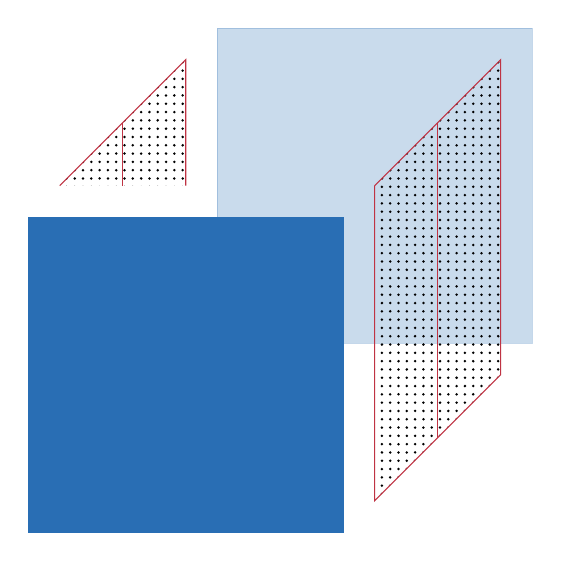
\begin{tikzpicture}[scale=4]
    \draw[spanish-blue, fill=spanish-blue] (0, 0) -- (1, 0) -- (1, 1) -- (0, 1) -- (0, 0);
    \draw[spanish-blue, fill=spanish-blue, nearly transparent] (0.6, 1) -- (0.6, 1.6) -- (1.6, 1.6) -- (1.6, 0.6) -- (1.0, 0.6);
    \draw[raspeberry, pattern=dots] (1.1, 1.1) -- (1.5, 1.5) -- (1.5, 0.5) -- (1.1, 0.1) -- (1.1, 1.1);
    \draw[raspeberry] (1.3, 1.3) -- (1.3, 0.3);
    \draw[raspeberry, pattern=dots] (0.1, 1.1) -- (0.5, 1.5) -- (0.5, 1.1);
    \draw[raspeberry] (0.3, 1.3) -- (0.3, 1.1);
  \end{tikzpicture}
  \;\;
  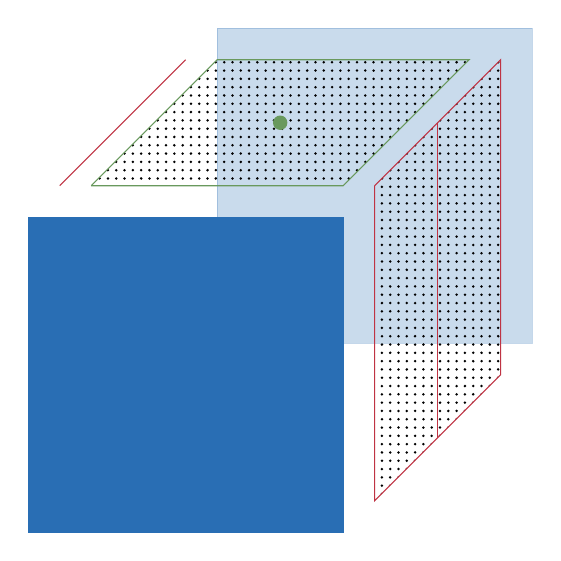
\begin{tikzpicture}[scale=4]
    \draw[spanish-blue, fill=spanish-blue] (0, 0) -- (1, 0) -- (1, 1) -- (0, 1) -- (0, 0);
    \draw[spanish-blue, fill=spanish-blue, nearly transparent] (0.6, 1) -- (0.6, 1.6) -- (1.6, 1.6) -- (1.6, 0.6) -- (1.0, 0.6);
    \draw[raspeberry, pattern=dots] (1.1, 1.1) -- (1.5, 1.5) -- (1.5, 0.5) -- (1.1, 0.1) -- (1.1, 1.1);
    \draw[raspeberry] (1.3, 1.3) -- (1.3, 0.3);
    \draw[raspeberry] (0.1, 1.1) -- (0.5, 1.5);
    \draw[russian-green, pattern=dots] (0.2, 1.1) -- (1.0, 1.1) -- (1.4, 1.5) -- (0.6, 1.5) -- (0.2, 1.1);
    \filldraw[russian-green] (0.8, 1.3) circle (0.6pt);
  \end{tikzpicture}
\end{center}

%%%%%%%%%%%%%%%%%%%%%%%%%%%%%%%%%%%%%%%%%%%%%%%%%%%%%%%%%%%%%%%%%%%%%%
\newpage

\begin{center}
\textcolor{red}{\huge The recursive construction, formally}
\end{center}
\vspace{-1mm}
\begin{large}
$$
\hspace{8mm}
\begin{array}{llcl}
\myfullbox{l}^{n} & (X_{<n}:\partialcubset{l}{n}) & : & \sort{l}\\
\myfullbox{l}^{n} & X_{<n} & \defeq & \mybox{l}^{n,n}(X_{<n})\\
\\
\mybox{l}^{n,p,[p \leq n]} & (X_{<n}:\partialcubset{l}{n}) & : & \sort{l}\\
\mybox{l}^{n,0} & X_{<n} & \defeq & \unittype\\
\mybox{l}^{n,p'+1} & X_{<n} & \defeq & \Sigma d:\mybox{l}^{n,p'}(X_{<n}).\,\mylayer{l}^{n,p'}(d)\\
\\
\mylayer{l}^{n,p,[p < n]} & \!\!\!\begin{array}{l}\{X_{<n}:\partialcubset{l}{n}\}~(d:\mybox{l}^{n,p}(X_{<n}))\end{array}& : & \sort{l}\\
\mylayer{l}^{n,p} & (X_{<n-1},X_{n-1})~d & \defeq & \Pi \epsilon.\,\mycube{l}^{n-1,p}(X_{n-1})(\downbox{l}{\epsilon}^{n,p}(d))\\
\\
\mycube{l}^{n,p,[p \leq n]} & \!\!\!\begin{array}{l}\{X_{<n}:\partialcubset{l}{n}\}~(X_n:\mycubsetcomp{l}{n}(X_{<n}))~(d:\mybox{l}^{n,p}(X_{<n}))\end{array}\!\!\! & : & \sort{l}\\
\mycube{l}^{n,p,[p = n]} & X_{<n}~X_n~d & \defeq & X_n(d)\\
\mycube{l}^{n,p,[p < n]} & X_{<n}~X_n~d & \defeq & \Sigma b:\mylayer{l}^{n,p}(d).\,\mycube{l}^{n,p+1}(X_n)(d,b)\\
\end{array}
$$
\end{large}
\noindent which corresponds, when $\nu=2$, to
the following organisation of the $3^n$ components of a $n$-cube (shown for $n=2$), with
$\mybox{l}$ associating layers on the left and $\mycube{l}$ associating them
on the right:
$$
\begin{array}{l}
\begin{array}{lll}
\mbox{\textit{squares}}\\
[3mm]\mbox{\textit{lines}}\\
[3mm]\mbox{\textit{points}}\\
[1mm]\end{array}
\framebox{$\begin{array}{lll}
\overbrace{\raisebox{0.05cm}{\framebox{$
\begin{array}{ll}
\raisebox{0cm}{\hspace{.5cm}{\scriptsize$\mylayer{l}^{1,0}$}}  & \framebox{$x_{0\star}$}\\
[1mm]\overbrace{\framebox{$x_{00}$}~\framebox{$x_{01}$}}&
\raisebox{-0.1cm}{{\scriptsize \hspace{0.1cm}$\mycube{l}^{1,0}\!\!\!\!\!\!\!\!$}}
\\
\end{array}
$}}~
{\raisebox{0.05cm}{\framebox{$
\begin{array}{ll}
\raisebox{0cm}{\hspace{.5cm}{\scriptsize$\mylayer{l}^{1,0}$}}  & \framebox{$x_{1\star}$}\\
[1mm]\overbrace{\framebox{$x_{10}$}~\framebox{$x_{11}$}}&
\raisebox{-0.1cm}{{\scriptsize \hspace{0.1cm}$\mycube{l}^{1,0}\!\!\!\!\!\!\!\!$}}
\end{array}
$}}}}^{\mylayer{l}^{2,0}}~
\stackrel{\raisebox{9.5mm}{$\framebox{$
\begin{array}{ll}
\raisebox{0cm}{\hspace{.5cm}{\scriptsize$\mylayer{l}^{2,1}$}} & \framebox{$x_{\star\star}$}\\
[1mm]\overbrace{\framebox{$x_{\star 0}$}~\framebox{$x_{\star 1}$}}&
\raisebox{-0.1cm}{{\scriptsize \hspace{0.1cm}$\mycube{l}^{2,1}\!\!\!\!\!\!\!\!$}}
\end{array}
$}
$}}{\raisebox{-0.4cm}{{\scriptsize \hspace{2.5cm}$\mycube{l}^{2,0}\!\!\!\!\!\!\!$}}}
\end{array}$}
~~~\parbox{3.5cm}{{\it additionally, each atomic component at dimension $n$ is a $\mycube{l}^{n,n}$}}\\
[-1mm]\qquad\qquad~~\xymatrix{ \ar@{<->}[rr] & & }\!\!\mbox{\normalsize $\mybox{l}^{1,1}$}
      \quad~~\xymatrix{ \ar@{<->}[rr] & & }\mbox{\normalsize $\mybox{l}^{1,1}$}\\
[-2mm]\qquad\qquad\xymatrix{ \ar@{<->}[rrrrrrrr] & & & & & & & & }\mbox{\normalsize$\mybox{l}^{2,1}$}\\
[-2mm]\qquad\qquad\xymatrix{ \ar@{<->}[rrrrrrrrrrr] & & & & & & & & & & & }\mbox{\normalsize$\mybox{l}^{2,2}$}\\
\end{array}
$$

%%%%%%%%%%%%%%%%%%%%%%%%%%%%%%%%%%%%%%%%%%%%%%%%%%%%%%%%%%%%%%%%%%%%%%
\newpage

\begin{center}
\textcolor{red}{\huge The recursive construction: restrictions (``faces'')}
\end{center}

\begin{large}
$$\hspace{-1cm}
\begin{array}{llcl}
\downbox{m}{\epsilon}^{n,q,p,[p \leq q < n]} & \!\!\!\begin{array}{l}\{X_{<n}:\partialcubset{m}{n}\}\\(d:\mybox{m}^{n,p}(X_{<n}))\end{array}& : & \mybox{m}^{n-1,p}(X_{<n-1})\\
\downbox{m}{\epsilon}^{n,q,0} & X_{<n}~\unitpoint & \defeq & \unitpoint\\
\downbox{m}{\epsilon}^{n,q,p'+1} & X_{<n}~(d,l) & \defeq & (\downbox{m}{\epsilon}^{n,q,p'}(d),\downlayer{m}{\epsilon}^{n,q,p'}(l))\\
\\
\downlayer{m}{\epsilon}^{n,q,p,[p < q < n]} & \!\!\!\begin{array}{l}\{X_{<n}:\partialcubset{m}{n}\}\\\{d:\mybox{m}^{n,p}(X_{<n})\}\\(l:\mylayer{m}^{n,p}(d))\end{array}& : & \mylayer{m}^{n-1,p}(\downbox{m}{\epsilon}^{n,q,p}(d))\\
\downlayer{m}{\epsilon}^{n,q,p} & (X_{<n-1},X_{n-1})~d~l & \defeq & \lambda\epsilon'.\,\overrightarrow{\cohbox{m}{\epsilon,\epsilon'}^{n,p,q,p}(d)}(\downcube{m}{\epsilon}^{n-1,q-1,p}(l_{\epsilon'}))\\
\\
\downcube{m}{\epsilon}^{n,q,p,[p \leq q < n]} & \!\!\!\begin{array}{l}\{X_{<n}:\partialcubset{m}{n}\}\\\{X_n:\mycubsetcomp{m}{n}(X_{<n})\}\\\{d:\mybox{m}^{n,p}(X_{<n})\}\\(c:\mycube{m}^{n,p}(X_n)(d))\end{array}& : & \mycube{m}^{n-1,p}(X_{n})(\downbox{m}{\epsilon}^{n,q,p}(d))\\
\downcube{m}{\epsilon}^{n,q,p,[p=q]} & X_{<n}~X_n~d~(l,\_) & \defeq & l_{\epsilon}\\
\downcube{m}{\epsilon}^{n,q,p,[p<q]} & X_{<n}~X_n~d~(l,c) & \defeq & (\downlayer{m}{\epsilon}^{n,q,p}(l),\downcube{m}{\epsilon}^{n,q,p+1}(c))\\
\\
\end{array}
$$
\end{large}

\noindent where $\cohbox{m}{\epsilon,\epsilon'}$ is a coherence proof and we
write $\overrightarrow{\cohbox{m}{\epsilon,\epsilon'}}$ for the
  rewriting of this proof from left to right

%%%%%%%%%%%%%%%%%%%%%%%%%%%%%%%%%%%%%%%%%%%%%%%%%%%%%%%%%%%%%%%%%%%%%%
\newpage

\begin{center}
\textcolor{red}{\huge The recursive construction: coherences}
\end{center}

$$
\begin{large}\hspace{-1cm}
\begin{array}{llcl}
\cohbox{m}{\epsilon,\epsilon'}^{\!\!\!\tiny\begin{array}{l}n,q,r,p\\\mbox{}[p \leq r < q < n]\end{array}} & \!\!\!\begin{array}{l}\{X_{<n}:\partialcubset{m}{n}\}\\(d:\mybox{m}^{n,p}(X_{<n}))\end{array}& : & \!\!\!\begin{array}{ll}\downbox{m}{\epsilon}^{n-1,q-1,p}(\downbox{m}{\epsilon'}^{n,r,p}(d)) \\ = \downbox{m}{\epsilon'}^{n-1,r,p}(\downbox{m}{\epsilon}^{n,q,p}(d))\end{array}\\
\cohbox{m}{\epsilon,\epsilon'}^{n,q,r,0} & X_{<n}~\unitpoint & \defeq & \refl{\unitpoint}\\
\cohbox{m}{\epsilon,\epsilon'}^{n,q,r,p'+1} & X_{<n}~(d,l) & \defeq & (\cohbox{m}{\epsilon,\epsilon'}^{n,q,r,p'}(d),\cohlayer{m}{\epsilon,\epsilon'}^{n,q,r,p'}(l))\\
\\
\cohlayer{m}{\epsilon,\epsilon'}^{\!\!\!\tiny\begin{array}{l}n,q,r,p\\\mbox{}[p < r < q < n]\end{array}} & \!\!\!\begin{array}{l}\{X_{<n}:\partialcubset{m}{n}\{\\\{d:\mybox{m}^{n,p}(X_{<n})\}\\(l:\mylayer{m}^{n,p}(X_{<n})(d))\end{array}& : & \!\!\!\begin{array}{ll}\downlayer{m}{\epsilon}^{n-1,q-1,p}(\downlayer{m}{\epsilon'}^{n,r-1,p}(l)) \\ = \downlayer{m}{\epsilon'}^{n-1,r-1,p}(\downlayer{m}{\epsilon}^{n,q,p}(l))\end{array}\\
\cohlayer{m}{\epsilon,\epsilon'}^{n,q,r,p} & X_{<n}~d~l & \defeq & \lambda\epsilon''.\,\cohcube{m}{\epsilon,\epsilon'}^{n-1,q-1,r-1,p}(l_{\epsilon''})\\
\\
\cohcube{m}{\epsilon,\epsilon'}^{\!\!\!\tiny\begin{array}{l}n,q,r,p\\\mbox{}[p \leq r < q < n]\end{array}} & \!\!\!\begin{array}{l}\{X_{<n}:\partialcubset{m}{n}\}\\\{X_n:\mycubsetcomp{m}{n}(X_{<n})\}\\\{d:\mybox{m}^{n,p}(X_{<n})\}\\(c:\mycube{m}^{n,p}(X_{<n})(X_n)(d))\end{array}& : & \!\!\!\begin{array}{ll}\downcube{m}{\epsilon}^{n-1,q-1,p}(\downcube{m}{\epsilon'}^{n,r,p}(c)) \\ = \downcube{m}{\epsilon'}^{n-1,r,p}(\downcube{m}{\epsilon}^{n,q,p}(c))\end{array}\\
\cohcube{m}{\epsilon,\epsilon'}^{n,q,r,p,[p=r]} & X_{<n}~X_n~d~(l,\_) & \defeq & \refl({\downcube{m}{\epsilon}^{n-1,q-1,p}(l_{\epsilon})})\\
\cohcube{m}{\epsilon,\epsilon'}^{n,q,r,p,[p<r]} & X_{<n}~X_n~d~(l,c) & \defeq & \!\!\begin{array}{l}(\cohlayer{m}{\epsilon,\epsilon'}^{n,q,r,p}(l),\;\cohcube{m}{\epsilon,\epsilon'}^{n,q,r,p+1}(c))\end{array}\\
\end{array}
\end{large}
$$

\bigskip

\noindent where we hide some coherences (such as proof-irrelevance of
equality in $\HSet$ or the identification of the equality on pairs as
a pair of equalities)

%%%%%%%%%%%%%%%%%%%%%%%%%%%%%%%%%%%%%%%%%%%%%%%%%%%%%%%%%%%%%%%%%%%%%%
\newpage

\begin{center}
\textcolor{red}{\huge Adding reflexivities}
\end{center}

\iffalse
\newcommand{\myreflset}{\textsf{reflSet}}

$$
\begin{array}{llcl}
\multicolumn{4}{c}{\mbox{\textsf{\textit{Degeneracy structure}}}}\\
\\
\mycubset{l} && : & \sort{l+1}\\
\mycubset{l} && \defeq & \mycubsetfrom{l}{0}(\star)\\
\\
\mycubsetfrom{l}{n} & (X_{<n}:\partialcubset{l}{n}) & : & \sort{l+1}\\
\mycubsetfrom{l}{n} & X_{<n} & \defeq & \Sigma X_n:\mycubsetcomp{l}{n}(X_{<n}).\,\mycubsetfrom{l}{n+1}(X_{<n},X_n)\\
\\
\multicolumn{4}{c}{\mbox{\textsf{\textit{Truncated $\nu$-sets}}}}\\
\\
\partialcubset{l}{n} && : & \sort{l+1}\\
\partialcubset{l}{0} && \defeq & \unittype\\
\partialcubset{l}{n'+1} && \defeq & \Sigma X_{<n}:\partialcubset{l}{n'}.\,\mycubsetcomp{l}{n}(X_{<n}))\\
\\
\mycubsetcomp{l}{n} & (X_{<n}:\partialcubset{l}{n}) & : & \sort{l+1}\\
\mycubsetcomp{l}{n} & X_{<n} & \defeq & \myfullbox{l}^{n}(X_{<n})\rightarrow \sort{l}\\
\end{array}
$$
\fi

We now set $\nu = 1$. For any $\mycubset{l}$, we define a stream of reflexivities:
$$
\begin{array}{lll}
\nu\textsf{reflSet}(X_{-1},X_0,...) ~~ \defeq \\
\quad \Sigma r_{-1}:\Pi d:\mathsf{frame}^{-1}.\,\Pi x:X_{-1}(d).\,X_0(\mathsf{reflframe}^{-1}(d),x).\\
\quad \Sigma r_0:\Pi d:\mathsf{frame}^0(X_{-1}).\,\Pi x:X_{0}(d).\,X_1(\mathsf{reflframe}^0(r_{-1})(d),x).\\
\quad \Sigma r_1:\Pi d:\mathsf{frame}^1(X_{-1},X_0).\,\Pi x:X_{1}(d).\,X_2(\mathsf{reflframe}^1(r_{-1},r_0)(d),x).\\
\quad ...
\end{array}
$$
where
$$\mathsf{reflframe}^n(r_{-1},...,r_{n-1}):\mathsf{frame}^n(X_{-1},...,X_{n-1})
\rightarrow \mathsf{frame}^{n+1,n}(X_{-1},...,X_{n})$$ computes the
$n$ first layers of the border of $r_{n}(d)(x)$, knowing that the last
layer is made of $x$ itself, so that
$(\mathsf{reflframe}^n(r_{-1},...,r_{n-1})(d),x)$ is a full frame (the matching map formerly called $M_r$),
that is of type $\mathsf{frame}^{n+1}(X_{-1},...,X_{n})$.

\bigskip

We also need two coherence conditions:
$$
\!\!\begin{array}{l}
\mathsf{idrestrreflframe}^n(r_{-1},...,r_{n-1}): \Pi d:\mathsf{frame}^n.\,\mathsf{restrframe}^{n,n}_n(\mathsf{reflframe}^n(r_{-1},...,r_{n-1})(d)) = d\\
\mathsf{cohrestrreflframe}^n_{p<n}(r_{-1},...,r_{n-1}): \Pi d:\mathsf{frame}^{n,p}.\,\\
~\,\mathsf{restrframe}^{n,p}_p(\mathsf{reflframe}^{n,p}(r_{-1},...,r_{n-1})(d)) =
\mathsf{reflframe}^{n-1,p}(r_{-1},...,r_{n-2})(\mathsf{restrframe}^{n-1,p}_p(d))
\end{array}
$$
where $\mathsf{reflframe}^{n,p}$ generalises $\mathsf{reflframe}^{n}$
to prefixes of $\mathsf{frame}^n$:
$$\mathsf{reflframe}^{n,p}(r_{-1},...,r_{n-1}):\mathsf{frame}^{n,p}(X_{-1},...,X_{n-1})
\rightarrow \mathsf{frame}^{n+1,p}(X_{-1},...,X_{n})$$

%%%%%%%%%%%%%%%%%%%%%%%%%%%%%%%%%%%%%%%%%%%%%%%%%%%%%%%%%%%%%%%%%%%%%%
\newpage

\begin{center}
\textcolor{red}{\huge Summary}
\end{center}

\bigskip
\begin{itemize}
\item A work in progress, machine-checking a model following the iterated parametricity translation in indexed form.

\item The addition of a reflexivity in the last direction is completed

\item To be done: permutations, $\Pi$-types, $\Sigma$-types, universes, ...

\item Also in progress: a more compact definition relying on
  finer-grain dependencies between the different components of the
  construction.

\end{itemize}
\end{sf}
\end{Large}
\end{document}
